\documentclass{article}

\usepackage{amsfonts}
\usepackage{amsmath}
\usepackage{amsthm}
\usepackage{algorithm}
\usepackage{algorithmic}
\usepackage{bm}
\usepackage{hyperref}
\usepackage{footmisc}
\usepackage{xcolor}
\DeclareMathOperator\E{\mathbb{E}}
\DeclareMathOperator\Var{\mathrm{Var}}
\def\R{\mathbb{R}}
\def\P{\mathcal{P}}
\usepackage{mathtools}
\DeclarePairedDelimiter\abs{\lvert}{\rvert}
\DeclarePairedDelimiter\norm{\lVert}{\rVert}
\DeclarePairedDelimiter\inner{\langle}{\rangle}
\def\red#1{\textcolor{red}{#1}}
\makeatletter
\newcommand{\algorithmicfunction}{\textbf{function}}
\newcommand{\algorithmicendfunction}{\algorithmicend\ \algorithmicfunction}
\newenvironment{ALC@func}{\begin{ALC@g}}{\end{ALC@g}}
\newcommand{\FUNCTION}[2][default]{\ALC@it\algorithmicfunction\ #2\ %
\textbf{:}%
\ALC@com{#1}\begin{ALC@func}}
\ifthenelse{\boolean{ALC@noend}}{
    \newcommand{\ENDFUNCTION}{\end{ALC@func}}
  }{
    \newcommand{\ENDFUNCTION}{\end{ALC@func}\ALC@it\algorithmicendfunction}
  }
\makeatother
\theoremstyle{definition}
\newtheorem{definition}{Definition}
\newtheorem{theorem}{Theorem}
\newtheorem{example}{Example}
\newtheorem{corollary}{Corollary}
\newtheorem{lemma}{Lemma}
\newtheorem{remark}{Remark}
\begin{document}
\title{draft}
\author{zhaofeng-shu33}
\maketitle
%整体思路:
%   0. 基于hierarchical structure 
%   1. 用B matrix 重新定义 MMI
%   2. 定义的背景,是对用KL divergence 原定义的近似
%   3. 新定义满足的性质, 可以用现有迭代算法解决
%   4. 计算fundamental partition 的原理和算法pseudo code
%   5. 简单的例子、算法实现与验证
%   6. B matrix 的近似,人工数据验证
%   7. Real data
%   8. 总结与展望
\section{Background}
Hierarchical clustering is a popular clustering method. It produces a semi-lattice structure of clusters. 
An information-theoretic approach to hierarchical clustering is formulated in \cite{ic}.

The idea of this formulation is as follows:

Suppose we have a set of random variables $Z_1, Z_2, \dots, Z_{\abs{V}}$ to be clustered, and for a given threshold $\gamma \in \mathbb{R}$, the set of clusters is defined as:
\begin{equation}
C_{\gamma}(Z_V) = \textrm{maximal}\{ B \in V \vert \abs{B} > 1, I(Z_B) > \gamma \}
\end{equation}

The above definition excludes the singleton element.

The key is how to define $I(Z_B)$, which is called the multivariate mutual information(MMI) for $\{Z_i | i \in B\}$.

\red{It is indeed hierachical if MMI satisfies certain properties.}

In literature \cite{ic}, the MMI is defined as 
\begin{align}
I(Z_V) & = \min_{\mathcal{P} \in \Pi'(V)} I_{\mathcal{P}}(Z_V) \label{eq:opI}\\
\label{eq:MMI_o} I_{\mathcal{P}}(Z_V) & = {1 \over \abs{\mathcal{P}} -1 } D\left(P_{Z_V}|| \prod_{C\in \mathcal{P}} P_{Z_C} \right) 
\end{align}

We give a different definition of MMI.
\begin{align}
I(Z_V) & = \min_{\mathcal{P} \in \Pi'(V)} I_{\mathcal{P}}(Z_V) \\
\label{eq:newDef}  I_{\mathcal{P}}(Z_V) & = {1 \over 2( \abs{\mathcal{P}} - 1) } \sum_{\substack{(i,j) \not\in C\\ C\in \mathcal{P}}} \norm{\widetilde{B}_{ij}}_F^2
\end{align}

$\widetilde{B}_{ij}$ is called divergence transfer matrix which comes from the information geometry theory.
%The set of clusters can be computed from the \textit{Dilworth truncation} as the finest partition (not include the singleton element) which minimize $h_{\gamma}(\mathcal{P}) %$ (a piecewise linear function about $\gamma$), where
%\begin{equation}
%h_{\gamma}(\mathcal{P}) = \sum_{C \in \mathcal{P}} h(C) - \gamma \abs{ \mathcal{P}} , \mathcal{P} \in \Pi(V)
%\end{equation}

%From the definition of multivariate mutual information,  $h(C)$ is the joint entropy function of random variables $Z_i, i\in C$.  If the model satisfies certain conditions, the %minimizer can be computed as the graph-cut function, which is also submodular.
\section{Origin}
Our definition \eqref{eq:newDef} comes from an approximation of equation \eqref{eq:MMI_o} under certain conditions.

See appendix \ref{sec:akld} for detail.
Let $w_{ij} = \norm{\widetilde{B}_{ij}}_F^2$.
$\norm{\widetilde{B}_{ij}}_F^2$ can be treated as a kind of similarity metric between two random variables.

The graph-cut weight is $\norm{\widetilde{B}_{ij}}_F^2$.

If we treat each index as a vertex in a graph, then the partition $\P$ divides these vertices into $\abs{\P}$ groups. 

\begin{align}
f(C) & = {1\over 2}\sum_{i\in C, j \in V\backslash C} w_{ij} \\
f_B(C) & = {1\over 2}\sum_{i\in C, j \in B\backslash C} w_{ij} \\
\end{align}
We can write 
\begin{align}
f[\P] & = \sum_{C \in \P} f(C) \\
I_{\mathcal{P}}(Z_V)  &= { 1 \over \abs{\P}  - 1}f(\P) 
\end{align}
%$f$ on $S_i$ is a submodular function defined as graph cut.

Below we show some properties of MMI.

\begin{description}
\item[$G$] graph $G(V,E)$, with vertex set $V$ and edge set $E$
\item[$\Pi$] collection of partitions, $\Pi = \Pi(V)$
\item[$\Pi_B$] collection of partitions, $\Pi_B = \Pi(B), B\subseteq V$
\item[$\P$] a partition of $V$, $\P \in \Pi$
\item[$\P_B$] a partition of $B$, $\P_B \in \Pi_B$
\item[$\Pi'$] non-trivial partitions $\Pi' = \Pi \backslash \{V\}$
\item[$\Pi'_B$] non-trivial partitions $\Pi' = \Pi_B \backslash \{V\}$
\item[$\P_1 \vee \P_2$] the least element of $\Pi$ above $\P_1$ and $\P_2$
\item[$\P_1 \wedge \P_2$] the greatest element of $\Pi$ below $\P_1$ and $\P_2$
\item[$f(\cdot)$] submodular function defined on subset of $V$. $\mathrm{Domain}(f)=\{C| C\subset V\}$
\item[$f_B(\cdot)$] submodular function defined on subset of $B\subseteq V$. $\mathrm{Domain}(f)=\{C| C\subset B\}$
\item[$f{[}\cdot{]}$] function defined on $\Pi$ by $f[\P] = \sum_{C\in \P} f(C)$
\item[$f_B{[}\cdot{]}$] function defined on $\Pi_B$ by $f_B[\P_B] = \sum_{C\in \P_B} f(C)$
\item[$h_{\lambda}(\P)$] function defined on $\Pi$ by $h_{\lambda}(\P)=f[\P]-\lambda\abs{\P}$
\item[$h(\lambda)$] function defined as $ h(\lambda) = \min_{\P \in \Pi'} h_{\lambda}(\P)$
\item[$x(\cdot)$] modular function defined on subset of $V$ where $x$ is a vector: $x(C)=\sum_{i \in C} x_i$
\item[$\preceq$] partial order on $\Pi$, $\P_2 \preceq \P_1$ means $C\in \P_2 \Rightarrow \exists C' \in \P_1 \,s.t.\, C \subset C'$
\item[$\prec$] in strict sense such that $\P_1 \neq \P_2 $
\item[$\P/\P'$] the partition of $\P$ by $\P'$, requiring $\P\preceq \P'$ and $\P/\P'=\{\{ C \in P | C \subseteq C' \} | C' \in \P'\}$
\end{description}


\begin{theorem}\label{thm:lattice_structure}
Let $f$ be a submodular function on the subset of $V$. Let $\P_1, \P_2$ be partitions
at which $f$ reaches its minimum. Then $f$ reaches a minimum at $\P_1 \vee \P_2$ and $\P_1 \wedge \P_2$.
\end{theorem}
\begin{proof}
See Theorem 3.5 of literature \cite{psp}.	
\end{proof}
\begin{theorem}\label{thm:hierarchical}
Let $f$ be a submodular function on the subset of $V$. Let $\P_1, \P_2$ be partitions
at which $h_{\lambda_i}(i=1,2)$ reaches its minimum. 
If $\lambda_1 < \lambda_2$, then $\P_2 \preceq \P_1$.
\end{theorem}
\begin{proof}
	See Theorem 3.7 of literature \cite{psp}.	
\end{proof}

\begin{example}
Let $\P_1 = \{\{1, 2\}, \{3\}, \{4\}\}$, $\P_2 = \{\{1,3\},\{2\},\{4\}\}$, $\P_1\vee \P_2 = \{\{1,2,3\},\{4\}\}$, $\P_1 \wedge \P_2 = \{\{1\},\{2\},\{3\}, \{4\}\}$
\end{example}
\begin{example}
Let $\P_1 = \{\{1\}, \{2\}, \{3\}\}$, $\P_2 = \{\{1,2\},\{3\}\}$, $\P_1 / \P_2 = \{\{\{1\},\{2\}\},\{\{3\}\}\}$.
\end{example}

\begin{lemma}\label{lem:ref_combination}
For any $B \in \P' \in \Pi'$ and $\P_B \in \Pi'_B$, let $\P = \P_B \cup \P' \backslash \{B\} $
be the refinement of $\P'$. Then we have
\begin{equation}\label{eq:ref_combination}
I_{\P}(Z_V) = \theta I_{\P'}(Z_V) + (1-\theta) I_{\P_B}(Z_B)
\end{equation}
\end{lemma}
\begin{proof}
First we have $\abs{\P} = \abs{\P'} -1 + \abs{\P_B}$,
Since
\begin{align*}
I_{\P}(Z_V) & = { f[\P'] + f_B[\P_B] \over \abs{\P} - 1} \\
I_{\P'}(Z_V) & = { f[\P'] \over \abs{\P'} - 1} \\
I_{\P_B}(Z_B) & = { f_B[\P_B] \over \abs{\P_B} - 1}
\end{align*}
As a result, there exists $\theta = {\abs{\P'} - 1 \over \abs{\P} - 1} \in (0,1)$ such that 
\eqref{eq:ref_combination} holds.
\end{proof}
\begin{lemma}\label{lem:mi_split}
For any $\P:=\{C_1, \dots, C_k\} \in \Pi'$, we have
\begin{align}
I_{\P}(Z_V) =& I(Z_{C_1} \wedge \dots \wedge Z_{C_k}) \label{eq:mmi_representation} \\
=& { 1 \over k-1} \sum_{i=1}^{k-1} I(Z_{C_i} \wedge Z_{\cup_{j=i+1}^k C_j}) \label{eq:mi_mmi}
\end{align}
\end{lemma}
\begin{proof}
$I(Z_1 \wedge Z_2)$ is a kind of representation of mutual information.
And we use \eqref{eq:mmi_representation} to represent the multivariate mutual information.

Equation \eqref{eq:mi_mmi} is true for $k=2$. Suppose it holds for $k=m$. Then
let $B=\{C_m, C_{m+1}\}$ , $\P=\{C_1, \dots, C_{m+1}\}$
and use the result of lemma \ref{lem:ref_combination}, 
we have $\theta = \frac{m-1}{m}$
\begin{align*}
I(Z_{C_1} \wedge \dots \wedge Z_{C_{m+1}}) & = 
 \frac{m-1}{m} I(Z_{C_1} \wedge \dots \wedge Z_{C_m})
+ \frac{1}{m}  I(Z_{m} \wedge Z_{m+1}) \\
& = \frac{m-1}{m} \frac{1}{m-1}\sum_{i=1}^{m-1} I(Z_{C_i} \wedge Z_{\cup_{j=i+1}^m C_j})
+ \frac{1}{m}  I(Z_{m} \wedge Z_{m+1})\textrm{ by induction} \\
& = \frac{1}{m} \sum_{i=1}^{m} I(Z_{C_i} \wedge Z_{\cup_{j=i+1}^{m+1} C_j})
\end{align*}
\end{proof}
\begin{remark}
This lemma shows that we can use the mutual information to compute the multivariate mutual information.
\end{remark}
And then we show its connection with $h(\lambda)$.
\begin{theorem}\label{thm:f}
$I(Z_V)$ is the smallest value $\lambda$ that satisfies
\begin{equation}\label{eq:rir}
-\lambda = h_{\lambda}(\P)
\end{equation}
for some $\P \in \Pi'(V)$. Let $\Pi^*$ be the set of all such partitions satisfying \eqref{eq:rir}.
\end{theorem}
\begin{proof}
$I(Z_V)$ satisfies equation \eqref{eq:rir} for some $\P$. We only need to show the equality never holds for $\lambda < I(Z_V)$ and all partition $\P$. Indeed, we show $-\lambda < h_{\lambda}(\P)$.
\begin{align*}
-\lambda < h_{\lambda}(\P) &\iff -\lambda < f[\P] - \abs{\P} \lambda \\
& \iff \lambda < { f[\P] \over \abs{\P} - 1 } \\
& \iff \lambda < \min_{\P \in \Pi'(V)} { f[\P] \over \abs{\P} - 1 } \\
& \iff \lambda < I(Z_V)
\end{align*}
\end{proof}
\begin{remark}
Geometrically speaking, we know that the first line segment of $h(\lambda)$ is $\lambda$, theorem \ref{thm:f} shows that $I(Z_V)$ is the first critical value of $h(\lambda)$. It is the x coordinate of the intersection point of $-\lambda$ and a line with slope large than 1. $\Pi^*(Z_V) $ are just the collection of partitions which minimize $h_{\lambda}(\P)$, we can also show that this collection coincides with the optimal partitions to \eqref{eq:opI}.
\end{remark}

\begin{corollary}\label{cor:F}
$\Pi^*= \{ P \in \Pi: I_{\P}(Z_V) = I(Z_V)\}$
\end{corollary}
\begin{proof}
Let $\gamma = I(Z_V)$
\begin{align*}
-\gamma = h_{\gamma}(\P) & \iff  \gamma = { f[\P] \over \abs{\P} - 1 } \\
& \iff I(Z_V) = I_{\P}(Z_V)
\end{align*}
\end{proof}

From corollary \ref{cor:F} and theorem \ref{thm:lattice}, we know that if $I(Z_V) = I_{\P_1}(Z_V) = I_{\P_2}(Z_V)$, then $I(Z_V) = I_{\P_1 \wedge \P_2}(Z_V)$. Then we have the theorem:
\begin{theorem}
There is a unique finest partition $\P^* \in \Pi^*$, referred to as the fundamental partition.
\end{theorem}
\begin{proof}
Since $\Pi^*$ has the lattice structure, the meet of all its member is the unique finest partition $\P^*$
\end{proof}
\begin{theorem}\label{thm:strict_larger_mi}
The fundamental partition $\P^*$ with the singletons removed is the set of all maximal subsets $B \subseteq V$ with strictly larger mutual information. 
That is, we have
\begin{enumerate}
\item $I(Z_B) > I(Z_V)$ for $B \in \P^*, \abs{B}>1$.
\item $I(Z_V) \geq I(Z_B)$ if $\exists \P_B \subseteq \P^*$.
\item If $I(Z_C) > I(Z_V)$, then $C\subseteq B$ for $B \in \P^*$.
\end{enumerate}
\end{theorem}
\begin{proof}
\begin{enumerate}
\item
Suppose $I(Z_B)=I_{\P_B}(Z_B)$.
Let $\P' = \P_B \cup  \P^* \backslash \{B\}$.
Then $\abs{\P'} = \abs{\P^*} -1 + \abs{\P_B}$,
Since
\begin{align*}
I_{\P'}(Z_V) & = { f[\P^*] + f_B[\P_B] \over \abs{\P'} - 1} \\
I_{\P^*}(Z_V) & = { f[\P^*] \over \abs{\P^*} - 1} \\
I_{\P_B}(Z_B) & = { f_B[\P_B] \over \abs{\P_B} - 1}
\end{align*}
As a result, there exists $\theta = {\abs{\P^*} - 1 \over \abs{\P'} - 1} \in (0,1)$ such that 
\begin{equation}\label{eq:convexZ}
I_{\P'}(Z_V) = \theta I_{\P^*}(Z_V) + (1-\theta) I_{\P_B}(Z_B)
\end{equation}
Since $\P^*$ is finest, we have $I_{\P'}(Z_V) > I(Z_V)$, then from \eqref{eq:convexZ}, we have 
$I(Z_V) < \theta I(Z_V) + (1-\theta) I(Z_B) \Rightarrow I(Z_B) > I(Z_V)$.

\item Let $\P' = \{B\} \cup \P^*\backslash \P_B$, then $\P^* = \P_B \cup \P'\backslash\{B\}$ , similar to equation \eqref{eq:convexZ}, we have
\begin{equation}
I_{\P^*}(Z_V) = \theta I_{\P'}(Z_V) + (1-\theta) I_{\P_B}(Z_B)
\end{equation}
Since $\P^*$ is optimal partition, we have $I_{P^*}(Z_V) = I(Z_V), I_{\P'}(Z_V)\geq I(Z_V) \Rightarrow I(Z_V) \geq I_{\P_B}(Z_B) \geq I(Z_B)$ 
\end{enumerate}
\end{proof}


Below we show that not only the first critical values coincides of info-clustering problem and PSP problem, all their critical values 
and finest partitions coincide.

\section{property}
\subsection{relation to Dilworth truncation}
\begin{align}
I(Z_V) &= \max\{ \lambda \in \R_+: \lambda \leq f(\P)/(\abs{\P} - 1) \text{ for all partition } \P \in \Pi'(V)\} \\
& = \max\{ \lambda \in \R_+:  -\lambda \leq f(\P) - \abs{\P} \lambda \} \text{ for all partition } \P \in \Pi'(V)\} \\
\label{eq:Connection}& = \max\{ \lambda \in \R_+: -\lambda \leq h(\lambda)\}
\end{align}
where 
\begin{equation}\label{eq:hLambda}
h(\lambda) = \min_{\P} \sum_{C\in \P} (f(C)-\lambda)
\end{equation}
$h(\lambda)$ is the Dilworth truncation(DT) of the submodular function $f(C)$. $h(\lambda)$
is piecewise linear. For each turning point of line segments, the optimal partition forms a lattice. That is, if $\P_1$ and $\P_2$ are optimal partitions at $\lambda$, then $\P_1\vee \P_2$ and $\P_1 \wedge \P_2$ are also optimal partitions.

The connection of \red{MMI with DT} is through equation \eqref{eq:Connection}. More precisely, $I(Z_V)$
is the solution of equation $-\lambda = h(\lambda)$.

This connection is similar from RIR in literature \cite{ic}. We have $f(V)=0$ in our definition and the first line segement is $-\lambda$. Therefore
$(I(Z_V),  y_1)$ is the first turning point of $h(\lambda)$.

Therefore the set of optimal partition to achieve $I(Z_V)$ forms a lattice $\P^*(Z_V)$.

Similar to Theorem 5.2 in literature \cite{ska}, the finest partition $\P^*(Z_V)$ exists and is called the 
\textbf{fundamental partition}.

\subsection{Laminarity}
From theorem \ref{thm:strict_larger_mi}, we can show that
\begin{equation}\label{eq:P}
I(Z_{C_1 \cup C_2}) \geq \min\{ I(Z_{C_1}), I(Z_{C_2})\}
\end{equation}
From literature \cite{ic}, this property implies we can use the iteration method to compute the entire clustering
provided we can compute the first critical value and the first set of clusters.

By \eqref{eq:P}, we can show that the collection of all clusters $C(Z_V)$ forms a laminar family\footnote{Laminarity means that for any intersecting subsets, one is contained in the other}, i.e.
\begin{equation}
B_1 \cap B_2 \in \{\emptyset, B_1, B_2\}
\end{equation}

This implies the hierachical structure of the clustering solution.
\subsection{Computing first critical value via fundamental partitition}
Similar to Proposition 3.1 in literature \cite{ic}, we can compute $C_{\gamma_1}$ by computing $\P^*(Z_V)$
\begin{description}
\item[Uniqueness] Follows from submodularity of  $h(\lambda)$ defined in equation \eqref{eq:hLambda}
\item[Maximal] Theorem 5.3 in literature \cite{ska}
\end{description}
\red{Why}

\subsection{clustering by fundamental partition}
\begin{algorithm}
\begin{algorithmic}[1]
\REQUIRE Statistics of $Z_V$ sufficient for calculating \texttt{FundamentalPartition}$(B)$ for all $B \subseteq V:\abs{B}>1$
\ENSURE $\mathcal{S}$ is a list of $(I(Z_C),C)$ for $ C \in \mathcal{C}(Z_V)$, which gives
$\Gamma(Z_V) = \{ \gamma' | (\gamma', B) \in \mathcal{S}\} $ and $ \mathcal{C}_{\gamma}(Z_V)
= \mathrm{maximal}\{B | (\gamma', B) \in \mathcal{S}, \gamma' > \gamma \}$
\STATE $\mathcal{S},\mathcal{T} \leftarrow$ empty queues
\STATE enqueue $V$ to $\mathcal{T}$
\WHILE{$\mathcal{T}$ is non-empty}
\STATE $B \leftarrow $ dequeue $\mathcal{T}$
\STATE $(\gamma, \P) \leftarrow$\texttt{FundamentalPartition}$(B)$
\STATE enqueue $(\gamma, B)$ to $\mathcal{S}$
\STATE enqueue all non-singleton elemenets of $\P$ to $\mathcal{T}$
\ENDWHILE
\FUNCTION{\texttt{FundamentalPartition}$(B)$}
  \RETURN $(I(Z_B), \P^*(Z_B))$
\ENDFUNCTION
\end{algorithmic}
\end{algorithm}

The computation of fundamental partition is not easy.
\subsection{Hierarchical clustering by PSP}
We inspect the property of $h(\lambda)$ from \eqref{eq:hLambda}. Since $h(\lambda)$ is piecewise linear, it is characterised by its turning points where the slope changes.
At turning point $p_i$, the optimal solution to achieve $h(\lambda)$ forms a lattice $\Pi_i$.
Define $\mathcal{P}_i = \min \Pi_i$, i.e. the finest partition from $\Pi_i$. Then we can show that
$\Pi_1 \succ \Pi_2 \dots \succ \Pi_N$, where $\Pi_1$ is the fundamental partition of $Z_V$ and $\Pi_N$ contains singleton elements only.

We have the following conclusion
\section{Relation to PIN model}
In PIN(Pairewise Indepedent Network)(literatue \cite{pin}, see definition 2.1 and 2.2 for detail).
We can show that ($E$ is the edge set, $e \in C$ represents the edge $e$ is in the subgraph $C$)
\begin{align*}
\sum_{C \in \P} H(Z_C) - H(Z_V) & = \sum_{C \in \P} (\sum_{e \in C} H_e + \sum_{\substack{e = (u,v) \\ u \in C, v\not\in C }} H_e) - \sum_{e \in E} H_e \\
& = {1 \over 2}\sum_{C \in \P}  \sum_{\substack{e = (u,v) \\ u \in C, v\not\in C }} H_e
\end{align*}
Therefore, in PIN model, we have
\begin{equation}
I(Z_V) = \min_{ \P \in \Pi'(V)} \frac{ \sum_{C \in \P} c(\delta_{G}(C))}{2(\abs{\P} - 1 )}
\end{equation}
where $\delta_{G}(C) = \{e = (u, v) \in E | u \in C, v \not\in C\} $ and $c(A) = \sum_{e\in A} H_e$.
This is (4.21a) in literature \cite{ic}
\section{Difference to entropy formulation}
In literature \cite{ic}, the definition of MMI is based on the submodular function is $H(Z_C)$, which is the joint entropy. It has the nondeceasing property such that the larger $C$ is, the bigger value $H(Z_C)$ takes. However, in our formulation of MMI, we use the graph cut function, it does not have the monotonic property and $f(V) = 0$ from the definition. Therefore, our work is not a special case of literature \cite{ic} even through many conclusions are similar.

In PIN model, the two definitions coincide. But the PIN model has strong assumptions and is not practical. Our formulation of MMI is suitable to be applied directly to cluster cases in real work application.
\section{Contributions}
\begin{enumerate}
\item Use graph cut function to reformulate MMI.
\item Implement the algorithm in C++, which is fast and can be used by others.
\item The algorithm can be customized by using different similarity metric between two random variables.
\end{enumerate}
\appendix
\section{Approximation of KL Divergence}\label{sec:akld}
Suppose $U$ is uniformly distributed over $\{1, 2,\dots, 2K\}$, $X_1, \dots, X_n$ are independent conditioned on $U$.
Further suppose that each $X_i$ is weakly dependent with $U$.  That is, 
$$
P_{X_i | U=k}(x) = P_{X_i} (x)( 1 + \epsilon {\phi^{(k,i)}(x ) \over \sqrt{P_{X_i}(x)}} )
$$
Since 
\begin{align*}
P_{X_i}(x) &= \sum_{k=1}^{2K} P_{X_i | U=k}(x) P_U(k) \\
& = {1 \over 2K} \sum_{k=1}^{2K}P_{X_i} (x)( 1 + \epsilon {\phi^{(k,i)}(x ) \over \sqrt{P_{X_i}(x)}} )\\
\Rightarrow & \sum_{k=1}^{2K} {\phi^{(k, i)}(x) \over \sqrt{P_{X_i}(x)}} =0,\forall i, x\in \mathcal{X}
\end{align*}

Then
\begin{align*}
P_{X_1,\dots,X_n}(x_1,\dots,x_n)  &= \sum_{k=1}^{2K} P_{X_1,\dots,X_n | U=k}(x_1,\dots,x_n) P_U(k) \\
&= {1 \over 2K} \sum_{k=1}^{2K} \prod_{i=1}^n P_{X_i|U=k}(x_i)\\
&= {1 \over 2K} \sum_{k=1}^{2K} \prod_{i=1}^n P_{X_i|U=k}(x_i)\\
&= {1 \over 2K} \sum_{k=1}^{2K} \prod_{i=1}^n \left(P_{X_i} (x_i)( 1 + \epsilon {\phi^{(k,i)}(x_i ) \over \sqrt{P_{X_i}(x_i)}} )\right)\\
&= {1 \over 2K} \sum_{k=1}^{2K} (\prod_{i=1}^n  P_{X_i} (x_i))
\left( 1 + \epsilon\sum_{i=1}^n {\phi^{(k,i)}(x_i) \over \sqrt{P_{X_i}(x_i)}} + \epsilon^2\sum_{i\neq j}{\phi^{k,i}(x_i)\phi^{k,j}(x_j)\over \sqrt{P_{X_i}(x_i)P_{X_j}(x_j)} }\right)+o(\epsilon^2) \\
&= (\prod_{i=1}^n  P_{X_i} (x_i))
\left(1+{\epsilon\over 2K}\sum_{i=1}^n \sum_{k=1}^{2K}{\phi^{(k,i)}(x_i) \over \sqrt{P_{X_i}(x_i)}} +{\epsilon^2 \over 2K}\sum_{k=1}^{2K}\sum_{i\neq j}{\phi^{k,i}(x_i)\phi^{k,j}(x_j)\over \sqrt{P_{X_i}(x_i)P_{X_j}(x_j)} }\right) + o(\epsilon^2)\\
&= (\prod_{i=1}^n  P_{X_i} (x_i))
\left(1 +\sum_{i\neq j}{\epsilon^2 \over 2K}\sum_{k=1}^{2K}{\phi^{k,i}(x_i)\phi^{k,j}(x_j)\over \sqrt{P_{X_i}(x_i)P_{X_j}(x_j)} }\right) + o(\epsilon^2)
\end{align*}
If only two random variables are used, we have:
$$P_{X_i, X_j}(x_i, x_j) = P_{X_i}(x_i)P_{X_j}(x_j)\left(1+{\epsilon^2 \over 2K} \sum_{k=1}^{2K}{\phi^{k,i}(x_i)\phi^{k,j}(x_j)\over \sqrt{P_{X_i}(x_i)P_{X_j}(x_j)} } \right) \footnotemark$$
\footnotetext{no $o(\epsilon^2)$ here}
Let $\widetilde{B}_{ij}(x_i, x_j)={P_{X_i, X_j}(x_i,x_j) - P_{X_i}(x_i)P_{X_j}(x_j) \over \sqrt{P_{X_i}(x_i)P_{X_j}(x_j)}} $, then we have:
\begin{align*}
{\epsilon^2 \over 2K} \sum_{k=1}^{2K}{\phi^{k,i}(x_i)\phi^{k,j}(x_j)\over \sqrt{P_{X_i}(x_i)P_{X_j}(x_j)} } & = {P_{X_i, X_j}(x_i, x_j) - P_{X_i}(x_i)P_{X_j}(x_j) \over P_{X_i}(x_i)P_{X_j}(x_j)} \\
& = {\widetilde{B}_{ij}(x_i, x_j) \over \sqrt{P_{X_i}(x_i)P_{X_j}(x_j)} }
\end{align*}
Therefore, we have 
\begin{equation}
P_{X_1,\dots,X_n}(x_1,\dots,x_n) =  (\prod_{i=1}^n  P_{X_i} (x_i))\left ( 1 + \sum_{i\neq j}{\widetilde{B}_{ij}(x_i, x_j) \over \sqrt{P_{X_i}(x_i)P_{X_j}(x_j)} }\right) +o(\epsilon^2)
\end{equation}
Then $P_{X_1,\dots, X_n}$ is in the neighborhood of $P_{X_1}\dots P_{X_n}$ with $$\phi(x_1,\dots, x_n)=
\sqrt{P_{X_1}(x_1)\dots P_{X_n}(x_n)}\left(\sum_{i\neq j}{\widetilde{B}_{ij}(x_i, x_j) \over \sqrt{P_{X_i}(x_i)P_{X_j}(x_j)} }\right)+o(\epsilon^2)$$
\begin{align*}
D(P_{X_1,\dots, X_n}|| P_{X_1}\dots P_{X_n}) & ={1 \over 2} \sum_{x_1,\dots,x_n}\phi^2(x_1,\dots, x_n) \\
& = {1\over 2}\sum_{x_1,\dots,x_n} (\prod_{i=1}^n  P_{X_i} (x_i)) \left(\sum_{i\neq j}{\widetilde{B}_{ij}(x_i, x_j) \over \sqrt{P_{X_i}(x_i)P_{X_j}(x_j)} }\right)^2 +o(\epsilon^2) 
\end{align*}
From the definition of $\widetilde{B}_{ij}$, the above is the summation over $\norm{\widetilde{B}_{ij}}^2_F$(the coupling item is zero). Therefore we get the second order approximation:
\begin{equation}
D(P_{X_1,\dots, X_n}|| P_{X_1}\dots P_{X_n}) \approx  {1 \over 2} \sum_{i\neq j} \norm{\widetilde{B}_{ij}}^2_F 
\end{equation}
Let $\Pi$ be the partition of $V=\{1,2,\dots, n\}$. Then we can show that 
\begin{equation}
D(P_{X_V} || \prod_{C\in \Pi} P_{X_{C}}) \approx {1 \over 2}\sum_{\substack{(i,j) \not\in C\\ C\in \Pi}} \norm{\widetilde{B}_{ij}}_F^2
\end{equation}
Then the multivariate mutual information can be defined as:
\begin{equation}
I(Z_V) = \min_{\Pi} {1 \over 2( \abs{\Pi} - 1) } \sum_{\substack{(i,j) \not\in C\\ C\in \Pi}} \norm{\widetilde{B}_{ij}}_F^2
\end{equation}
Specifically, when $n=2$ we have 
\begin{equation}
I(X;Y) \approx {1 \over 2} \norm{\widetilde{B}_{XY}}_F^2
\end{equation}
let $B(x,y)=\frac{P_{X,Y}(x,y)}{\sqrt{P_X(x)P_Y(y)}}$, then we have $\widetilde{B}(x,y)=B(x,y)-\sqrt{P_X(x)P_Y(y)}$ and 
\begin{equation}
\norm{\widetilde{B}}_F^2 = \norm{B}_F^2 -1
\end{equation}
For continue random variables, we modify the summation notation with the integral notation.
\begin{align}
\norm{\widetilde{B}}_F^2 & = \int \frac{p^2(x,y)}{p(x)p(y)} dx dy \\
& = \E[\frac{P(X,Y)}{P(X)P(Y)}]
\end{align}
compared with the definition of mutual information $I(X;Y) =  \E[\log \frac{P(X,Y)}{P(X)P(Y)}] $,
there is some similarity.

\begin{example}\label{ex:rho}
Consider $(X,Y)$ conforms to multivariate distribution with correlation coeffient $\rho$, then
we can compute $\norm{B}_F^2 = \frac{1}{1-\rho^2}$ for $0\leq \rho < 1 $.
\end{example}


Quantity ${1 \over 2} \norm{\widetilde{B}_{XY}}_F^2$ can be estimated from H-score.
Let $\sigma_1 \geq \sigma_2 \dots \geq \sigma_n$ be the signular values of  $\widetilde{B}$,
then
\begin{equation}
{1 \over 2} \sum_{i=1}^k \sigma_i^2  = \displaystyle\sup_{f\in \R^k, g \in \R^k} \E_{XY}[f^T(X)g(Y)]- {1 \over 2} \mathrm{tr}(\Lambda_{f(X)} \Lambda_{g(Y)})
\end{equation}
Take proper $k$ we can get at least \textbf{lower bound} of ${1 \over 2} \norm{\widetilde{B}_{XY}}_F^2$.

We use the above method to get h-score and compare it to the method:

\begin{table}[!ht]
\centering
\begin{tabular}{ccc}
\hline
$\rho$ & theoretical & empirical \\
\hline
0.1 & 0.01 & 0.01 \\
0.5 & 0.33 & 0.27 \\
0.9 & 4.26 & 0.78 \\
\hline
\end{tabular}
\end{table}


\section{Algorithm Architecture}
\begin{figure}[!ht]
\centering
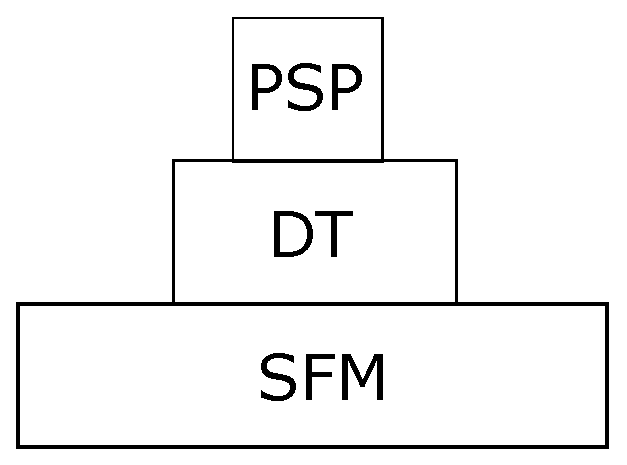
\includegraphics[width=5cm]{pic/pyramid.eps}
\caption{pyramid structure of info-clustering algorithm}\label{fig:ps}
\end{figure}
We use method of principal sequence of partition(PSP) to implement the info-clustering algorithm. As figure \ref{fig:ps} shows, PSP is at the highest level of algorithm pyramid. By divide and conquer technique, PSP calls at most $\abs{V}$ times of so-called Dilworth truncation(DT) algorithm. The relationship between PSP and DT is shown in Algorithm \ref{alg:psp}.
\begin{algorithm}
\caption{PSP algorithm}\label{alg:psp}
\begin{algorithmic}[1]
\REQUIRE Statistics of $Z_V$ sufficient for calculating $f(B)$ for all $B \subseteq V$
\ENSURE The array \textbf{L} contains the values in $\Gamma(Z_V)$. The array \textbf{PSP} contains the PSP $\P_1,\dots, P_N$. More specificly, $\textbf{PSP}[\abs{\P_i}]=\P_i, L[\abs{\P_{i-1}}]=\gamma_i$
\STATE \textbf{L}, \textbf{PSP} $\leftarrow$ empty arrays of size $\abs{V}$
\STATE $Q\leftarrow \{V\}, P \leftarrow \{ \{i \} | i \in V\}$
\STATE $\mathbf{PSP}[\abs{Q}]=Q, \mathbf{PSP}[\abs{P}] = P$
\STATE \texttt{Split}$(Q,P)$
\FUNCTION{\texttt{Split}$(Q,P)$}
 \STATE\label{alg:gamma} $\gamma' = {1 \over \abs{P} - \abs{Q}} (f(P)-f(Q))$
 \STATE $h' = {1 \over \abs{P} - \abs{Q}}(\abs{P} h(Q) - \abs{Q} h(P))$
 \STATE $(\tilde{h}, P') = \texttt{DT}(f,\gamma')$
 \IF{$\tilde{h}>h'$}
 	\STATE $\mathbf{L}[\abs{Q}] = \gamma'$
 \ELSE
 	\STATE $\mathbf{PSP}[\abs{P'}]=P'$
 	\STATE \texttt{Split}$(Q,P')$
 	\STATE \texttt{Split}$(P',P)$
 \ENDIF
\ENDFUNCTION
\end{algorithmic}
\end{algorithm}

In Algorithm \ref{alg:psp}, the function \texttt{Split} first calculates the intersection point of two lines: $f(P)-\abs{P}\lambda$ and $f(Q)-\abs{Q}\lambda$(in line~\ref{alg:gamma}) and then calls the DT algorithm to get the minimal value and minumal partition at $\gamma'$. From literature \cite{mac}, when there is partition between $Q$ and $P$, the $Split$ algorithm recursively calls itself to calculate all partitions.

For the middle level(DT) in the pyramid, it calls at most $\abs{V}$ times submodular function minimization(SFM) algorithm.
The algorithm is the same with procedure \texttt{FINDPARTITION} from literature \cite{mac}.

Actually, it uses Edmonds' greedy algorithm to finish this task. Consider the polyhedron defined by $f_{\lambda}(C) = f(C)-\lambda$($h_{\lambda}(\P)= \sum_{C \in \P} f_{\lambda}(C)$):
\begin{equation}
P(f_{\lambda}) = \{ x \in \R |  x(C) \leq f_{\lambda}(C), \emptyset \neq \forall C \subseteq V\}
\end{equation}

A non-empty set $C$ is called \textit{tight} for a vector $x \in P(f_{\lambda})$ if $x(C) = f_{\lambda}(C)$.
If we can find a vector $ x^* \in P(f_{\lambda}) $ and a complete partition $\P^*$ containing only tight partitions,
then $\P$ satisifies
\begin{align*}
h_{\lambda}(\P^*) &= \sum_{C \in \P^*} f_{\lambda}(C) \\
 &=\sum_{C\in P^*} x^*(C)  \\
& = \sum_{C \in \P} x^*(C), \forall \P \subset \Pi(V) \\
& \leq \sum_{C\in \P} f_{\lambda}(C), \textrm{since } x^* \in P(f_{\lambda}) \\
& = h_{\lambda}(\P),\forall \P \subset \Pi(V) 
\end{align*}

Let $V=\{1, 2, \dots, n\}$, the greedy algorithm to find $x^*$ and $\P^*$ is given in \ref{alg:dt}
\begin{algorithm}
\caption{Dilworth truncation algorithm(\texttt{DT})}\label{alg:dt}
\begin{algorithmic}[1]
\REQUIRE function $f$ and $\lambda$ which are requirements in the definition of $h_{\lambda}(\P)$.
\ENSURE the partition $\P^*$ s.t. $h(\lambda) = h_{\lambda}(\P^*)$ and the value of $h(\lambda)$
\STATE $V^0 = \emptyset, x = $ \texttt{zero vector}, $\mathcal{A} = $ \texttt{empty partition} 
\FOR{$l=1, 2, \dots, n$}
\STATE $V^l = \{l\} \cup V^{l-1}$
\STATE\label{alg:tight} compute $x^*_l = \displaystyle\min_{ A: l \in A \subseteq V^l} f_{\lambda}(A)- x(A)$ and $T^l$ is one of the minimizer.
\STATE $U^l = T^l \cup [\cup \{A | A \in \mathcal{A}, A \cap T^l \neq \emptyset\}] $
\STATE $\mathcal{A} = \{U^l\} \cup \{A | A \in \mathcal{A}, A \cap T^l = \emptyset \}$
\ENDFOR
\STATE $\P^* = \mathcal{A}, h_{\lambda} = x^*(V)$
\end{algorithmic}
\end{algorithm}

In line \ref{alg:tight} of Algorithm \ref{alg:dt}, the set $T^l$ remains tight.

SFM algorithm has been proved to have combinatorial polynomial time algorithm. However, in applications provable combinatorial algorithm for SFM does not perform well. General implementation like Fujishige-Wolfe minimum norm algorithm( in literature \cite{fwrobust}) fails because of intracable accuracy.
To finish our job, we focus on the specific problem to minimize 
\begin{equation}
\alpha^l = \min \{ f(S) - x^{l-1}(S) - \lambda: l \in \forall S \subset V^l\}
\end{equation}
When $f(S)$ is digraph cut function, we can convert the problem to minimum $s-t$ cut problem(in Algorithm 2, literature \cite{pin}). 
\begin{equation}
\beta^l = \min_{T \subseteq V^l \backslash \{s\}: l \in T} c(V^l \backslash T, T)
\end{equation} 

The optimal solution matches while the optimal values differs a constant value. 
\begin{equation}
\beta^l - \alpha^l = \lambda + \sum_{x_v>0, 1\leq v<l}x_{v}
\end{equation} 
\subsection{Example}

In this subsection, we use an illustrative example to explain the algorithm pyramid.
The first simulation setting(Fig~\ref{fig:4p}) is the same with subsection 5.1 in \cite{mac}.  We use principal sequence of partition to obtain the following result.
Aslo, figures on the same line are from one execution of \texttt{split}.

In the second simulation environment(Fig~\ref{fig:3c}), we generate 60, 100, 140 points uniformly on three circles and 10 random points on the line segment. The similarity metric is based on the polar coordinates of each point.

\begin{figure}[!ht]
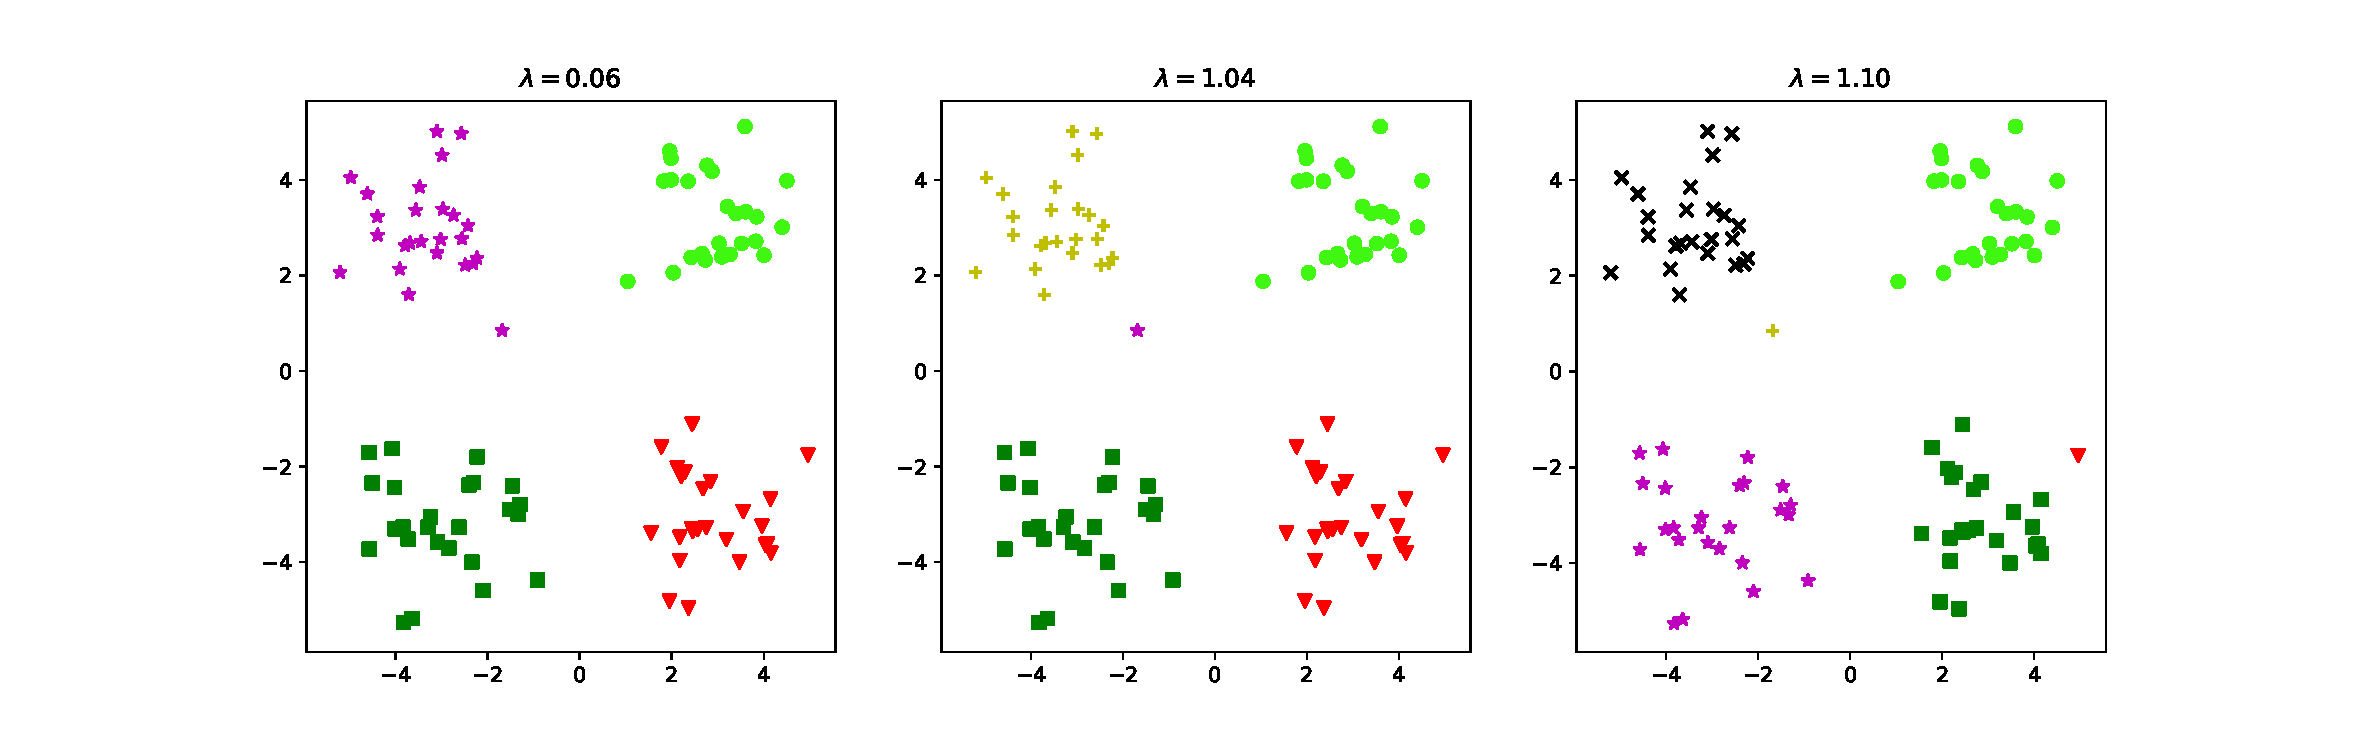
\includegraphics[width=12cm]{pic/4part.eps}
\caption{Illustrative example from four Gaussians}\label{fig:4p}
\end{figure}

\begin{figure}[!ht]
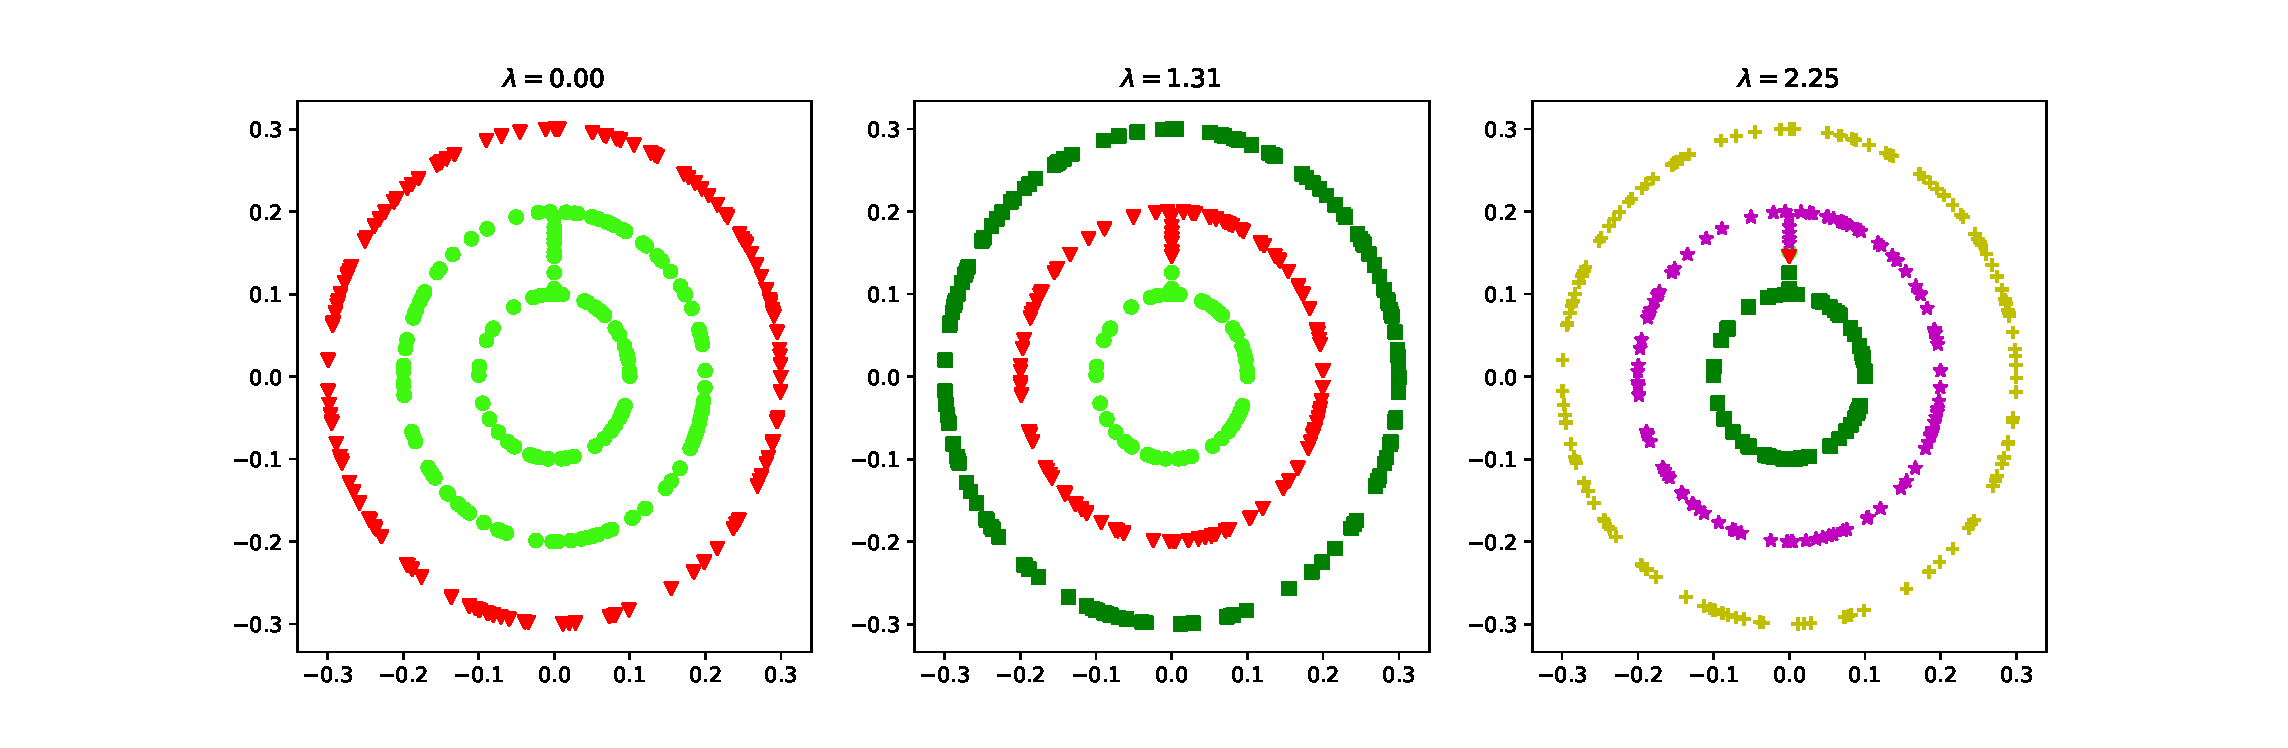
\includegraphics[width=12cm]{pic/3circle.eps}
\caption{Illustrative example from three circles}\label{fig:3c}
\end{figure}
\subsection{Comparision with other clustering method}
In this section, we use 4 different clustering methods and test them on 5 different datasets. The clustering methods are kmeans, spectral clustering, affine propagation and our info-clustering algorithms. We use adjusted rand score as accuracy criterion. The 5 datasets are 4 Gaussian blobs, 3 circles and the other three are from UCI datasets(Iris, Glass and Libras).
\begin{table}[!ht]
\centering
\InputIfFileExists{build/compare.tex}{}{}
\caption{clustering accuracy for the proposed and existing algorithms}
\end{table}
\subsection{Outlier detection}
\begin{thebibliography}{9}
\bibitem{ic}Info-Clustering: A Mathematical Theory for Data Clustering
\bibitem{ska} Multivariate Mutual Information Inspired by Secret-Key Agreement
\bibitem{pin} Info-Clustering: An Efficient Algorithm by Network Information Flow
\bibitem{mac} Minimum Average Cost Clustering
\bibitem{fwrobust} Provable Submodular Minimization using Wolfe's Algorithm
\end{thebibliography}
\end{document}
